\subsection{Számolások}
\includepdf[pages=-]{pdfs/iir.pdf}

\subsection{Python ellenőrzés}

A kézzel számolt értékeket bevezettem Python-ba és kirajzoltam az átviteli függvény Bode diagramját. Az összehasonlításért a Scipy modult használva kirajzoltam a modul által tervezett szűrő Bode diagramját.

\begin{figure}[H]
    \centering
    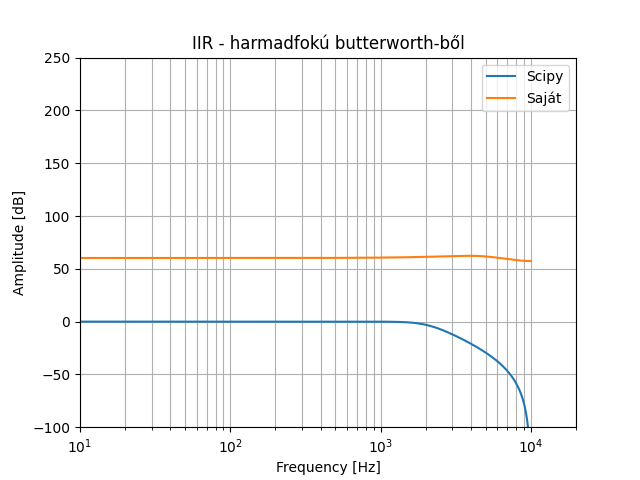
\includegraphics[scale=0.7]{figures/bode.png}
    \caption{Bode diagram kiszámolt és Scipy által tervezett IIR}
\end{figure}

A kézzel tervezett szűrő közel sem áll egy alul-áteresztő szűrőhöz. A számításokat többször leellenőriztem, viszont nem kaptam hibát. Mivel az IIR szűrő tervezésénél stabilitásprobléma léphet fel, úgy véltem az lehet a probléma. Kirajzoltam a rendszer pólusait és azt láttam, hogy ez valóban instabil (az egyik pólus az egységsugarú körön kívül van).

\begin{figure}[H]
    \centering
    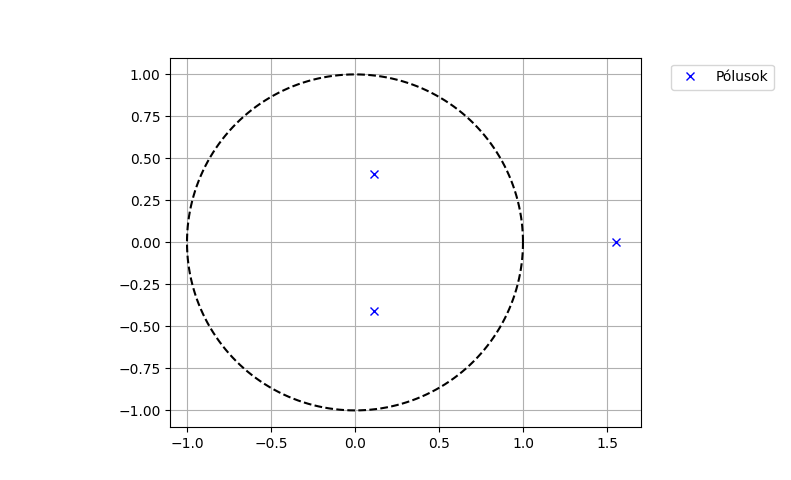
\includegraphics[scale=0.6]{figures/poles.png}
    \caption{Stabilitás vizsgálata}
\end{figure}

